\chapter{Asking Dubai Supercar Owners How They Got RICH!}

In this School of Hard Knocks interview, curated by LazyingArt LLC, the visible object is a supercar, but the real subject is commercial method. The lecture begins with spectacle and only later earns its abstractions: first we are shown a Rolls-Royce, a water-park empire, Jason Derulo, hundreds of millions, and a claim about cash purchases in Dubai; only afterward do we work our way down into partner risk, repeated rejection, land-backed businesses, negotiation posture, and finally a compact but genuinely mathematical warning about the destruction of compounding by recurring drag. The natural way to read the chapter is therefore not as a catalogue of rich people, but as a sequence of increasingly explicit models of how wealth is built, defended, and sometimes silently eroded.

\section{Dubai as Cold Open}

The lecture does not start by explaining anything. It starts by arranging a set of magnitudes in front of us: a Rolls-Royce, a business owner with the world's largest water park, Jason Derulo making \(\$30\) million in a year, another owner speaking of hundreds of millions, and a Dubai purchase made in cash. The point of the opening is structural. We are first asked to see the finished object, and only later to ask what chain of business decisions could possibly support it.

One of the first concrete quantities is the price of the Rolls-Royce:
\begin{equation}
C_{\text{Rolls}}=\$600{,}000.
\end{equation}
The lecture uses that number in two ways at once. On the surface, it works as a shock device. Underneath, it sets up a question about transaction form. If a car at that scale is bought in cash, then the interesting thing is no longer the car itself but the financial environment in which such a purchase feels ordinary.

\begin{figure}[h]
\centering
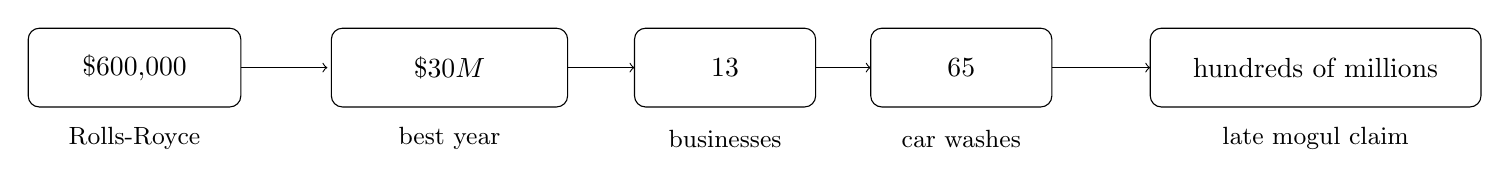
\begin{tikzpicture}[x=1cm,y=1cm]
\node[draw, rounded corners, minimum width=2.7cm, minimum height=1cm] (a) at (0,0) {\(\$600{,}000\)};
\node[draw, rounded corners, minimum width=3cm, minimum height=1cm] (b) at (4,0) {\(\$30\text{M}\)};
\node[draw, rounded corners, minimum width=2.3cm, minimum height=1cm] (c) at (7.5,0) {\(13\)};
\node[draw, rounded corners, minimum width=2.3cm, minimum height=1cm] (d) at (10.5,0) {\(65\)};
\node[draw, rounded corners, minimum width=4.2cm, minimum height=1cm] (e) at (15,0) {hundreds of millions};

\node at (0,-0.9) {\small Rolls-Royce};
\node at (4,-0.9) {\small best year};
\node at (7.5,-0.9) {\small businesses};
\node at (10.5,-0.9) {\small car washes};
\node at (15,-0.9) {\small late mogul claim};

\draw[->] (1.35,0) -- (2.45,0);
\draw[->] (5.5,0) -- (6.35,0);
\draw[->] (8.65,0) -- (9.35,0);
\draw[->] (11.65,0) -- (12.9,0);
\end{tikzpicture}
\caption{Transcript-based reconstruction of the lecture's cold open: price tags, income claims, and business counts are stacked before any mechanism is explained.}
\end{figure}

Once this opening collage has done its work, the host resets the scene: we are in Dubai, we will move through wealthy districts, and we will ask owners what they actually did to afford the machines in front of us. That reset matters. Without it, the lecture would remain a montage. With it, the lecture becomes an inquiry into business structure.

\section{The Water-Park Operator: Failure Counted Rather Than Hidden}

The first full case immediately refuses the easy reading of visible wealth. The host stops a G-Wagon owner, and within moments the conversation has moved from surface luxury to business adversity. The owner says he has been in business for more than a decade, that he owns the world's largest water park, and that he has been bankrupt twice and sued twenty-four times. Those are not decorative biographical details. They are the lecture's first serious move away from glamour and toward mechanism.

We can summarize the adversity count as
\begin{equation}
N_{\text{bankruptcies}}=2,
\qquad
N_{\text{lawsuits}}=24.
\end{equation}
A little later the numerical pressure becomes sharper:
\begin{equation}
D_{\text{negative}}\approx -\$1.8\,\text{million}.
\end{equation}
He describes a text message showing him \(\$1.8\) million in the hole, then says that for four years he was paying back debts created with a partner. At that point the lecture has already made two claims that matter for the chapter. First, partner choice is not a side issue; it is treated as a first-order business variable. Second, surviving a bad partnership can become part of the later operating doctrine.

The speaker prefers solo control now, even though he still does joint ventures. The reason is not abstract theory. It is memory. He describes himself as aggressive, open to failure, even comfortable with losing money in a way that many partners are not. Hence the underlying mismatch is not merely legal or financial. It is temperamental.

\subsection{Question \& Answer}

\paragraph{Question.}
How does repeated failure become business capital rather than a stopping point?

\paragraph{Answer.}
The lecture's answer is not sentimental. Failure becomes usable only when the operator does not treat it as a final verdict. Bankruptcy, lawsuits, and partner damage are not described here as honorable scars; they are described as expensive training. The speaker's compressed doctrine is that money can be remade, but the willingness to continue after public and financial damage is rarer. That is why he can say, almost coldly, that for him it is ``just money'' and that he knows what it feels like both to have money and not have it.

The lecture then tightens the same doctrine numerically through rejection:
\begin{equation}
N_{\text{rejections}}=617.
\end{equation}
If we spread that evenly across a year, we obtain the back-of-the-envelope rate
\begin{equation}
r_{\text{rejections}}
\approx
\frac{617}{365}
\approx
1.69\ \text{per day}.
\end{equation}
The speaker and host both round the idea upward into a daily rhythm of at least two no's. The exact average is less important than the shift in perspective: no is counted, not dramatized.

We can write the lecture's implicit update rule schematically as
\begin{equation}
\text{attempt}\to \text{no}\to \text{learning}\to \text{next attempt}.
\end{equation}
The exchange briefly garbles the usual slogan, but the intended meaning is plain: rejection is not evidence that the project is impossible; it is part of the search process.

A second layer of the same case arrives when he recalls a note written to himself eight years earlier, under three legal cases and roughly a quarter million dollars in debt:
\begin{equation}
D_{\text{note}}\approx -\$250{,}000.
\end{equation}
The note is not mathematics, but it functions like a self-imposed operating manual. Its commands are simple and severe: train the mind, refuse other people's limitations, accept pain, visualize, learn overload, become obsessed, never become satisfied. The lecture is careful here. Skill can be learned; discipline has to be carried.

Before leaving the case, the host performs an important recap. He says, in effect, that the Middle East is too easily read through a crude inheritance myth. The water-park operator is offered as a corrective: not born rich, not carried by family wealth, but built through repeated refusal to stop. That recap is not filler. It resets the audience's causal model before the next owner appears.

\section{Cash, Sacrifice, and the Social Price of Ambition}

The next full owner returns us to the Rolls-Royce, but not to the same lesson. This entrepreneur says he owns a fashion brand called Icon, has been an entrepreneur for six years, and made \(\$30\) million this year:
\begin{equation}
Y_{\text{fashion}}=\$30\,\text{million}.
\end{equation}
The host then asks the natural Dubai question: was the car bought in cash? The answer is yes, followed by the local framing that in Dubai many transactions happen in cash. The same \(\$600{,}000\) figure now reappears not merely as a price tag but as evidence of a transactional culture.

If the first case was about surviving failure, this second case is about paying for transformation. The speaker's central line is that we may have what we want if we are willing to bleed for it. The lecture does not leave that phrase floating. It unpacks it into concrete acts of renunciation: monk mode, isolation, reduced social life, indifference to short-term pleasures, and an explicit willingness to sacrifice the present self for the future one. The principle is not vague motivation. It is exchange.

\subsection{Question \& Answer}

\paragraph{Question.}
What price does the desired future extract from the present self?

\paragraph{Answer.}
The lecture's answer is that the price is not only monetary. The desired future competes with habits, friendships, romance, comfort, and immediate self-recognition. The speaker says everything has a price and that dream life has a price too. In other words, ambition is not merely additive. It is also subtractive. We become one thing partly by refusing to remain another.

That same logic extends outward into the social field. Haters are treated as structurally normal, not accidental. In the speaker's view, people often attack what they themselves gave up on. The result is a recurring theme of the lecture: social resistance is not evidence that the project is wrong; it is often one of the prices paid for staying with it. Here again the host does not ask us to admire the car. He asks us to think about the cost basis of the life that produced it.

At this point the lecture briefly breaks for a plug of the host's community and its mentors. That interruption should not be mistaken for part of the chapter's central doctrine, but it does matter rhythmically. It lowers the emotional pitch and resets the tempo before the celebrity case begins.

\section{Jason Derulo and the Car-Wash Machine}

Jason Derulo enters the lecture first as recognition and only then as mechanism. The host asks for the biggest amount made in a year, and the answer is again \(\$30\) million:
\begin{equation}
Y_{\text{Jason}}=\$30\,\text{million}.
\end{equation}
He then says he owns about thirteen businesses:
\begin{equation}
N_{\text{businesses}}\approx 13.
\end{equation}
The real reveal comes when the host asks which business made the most money. The answer is not music. It is car washes. The count is substantial:
\begin{equation}
N_{\text{car washes}}\approx 65.
\end{equation}

This matters because the lecture suddenly becomes more explicit about business structure. Car washes are profitable, he says, because they are a piece of land and because they generate money every day. People repeatedly wash their cars. The car itself stands in for personal presentation and visible success. Even during the pandemic, he says, people kept washing them. On top of that, the underlying real estate appreciates in value. Finally, superior customer service and attention to detail raise the quality of the operating asset.

The lecture does not supply a full underwriting model, so we should not invent one. But the logic can be summarized schematically as
\begin{equation}
V_{\text{car wash}}
\approx
V_{\text{land}}
+
V_{\text{recurring demand}}
+
V_{\text{service reputation}}.
\end{equation}
That equation should be read as a map of the speaker's explanation, not as a formal valuation identity. The key point is that the asset earns on two clocks at once. It throws off repeated operating revenue while also sitting on appreciating land.

\begin{figure}[h]
\centering
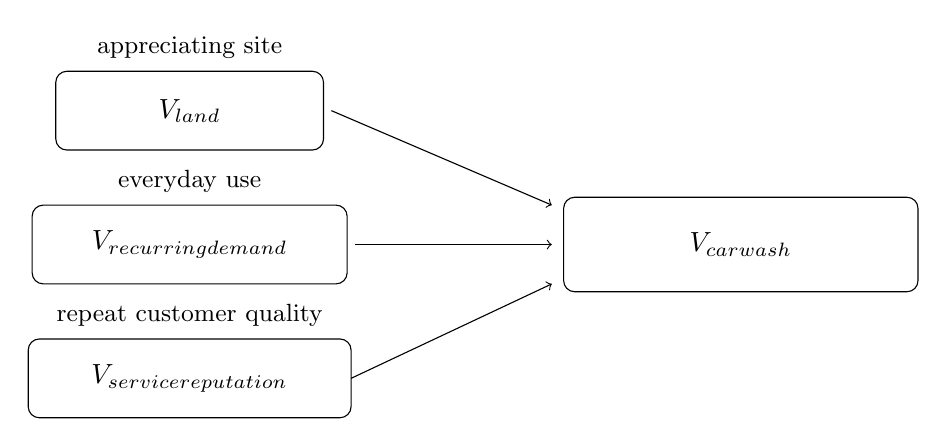
\begin{tikzpicture}[x=1cm,y=1cm]
\node[draw, rounded corners, minimum width=3.4cm, minimum height=1cm] (land) at (0,0) {\(V_{\text{land}}\)};
\node[draw, rounded corners, minimum width=4cm, minimum height=1cm] (demand) at (0,-1.7) {\(V_{\text{recurring demand}}\)};
\node[draw, rounded corners, minimum width=4.1cm, minimum height=1cm] (service) at (0,-3.4) {\(V_{\text{service reputation}}\)};
\node[draw, rounded corners, minimum width=4.5cm, minimum height=1.2cm] (total) at (7,-1.7) {\(V_{\text{car wash}}\)};

\draw[->] (1.8,0) -- (4.6,-1.2);
\draw[->] (2.1,-1.7) -- (4.6,-1.7);
\draw[->] (2.05,-3.4) -- (4.6,-2.2);

\node at (0,0.8) {\small appreciating site};
\node at (0,-0.9) {\small everyday use};
\node at (0,-2.6) {\small repeat customer quality};
\end{tikzpicture}
\caption{Transcript-based reconstruction of the car-wash case. The lecture treats the business as a combination of land, repeated use, and customer-experience quality.}
\end{figure}

\subsection{Question \& Answer}

\paragraph{Question.}
Why can a boring, land-backed business outperform glamour?

\paragraph{Answer.}
Because glamour is not itself a revenue model. The car-wash case is powerful precisely because it sounds unglamorous. The lecture's claim is that repetition, habit, and land can outrun celebrity aesthetics. If a business is tied to everyday behavior, generates cash repeatedly, and sits on an asset that appreciates, then it may be more durable than the glamorous career that first made the operator famous.

The speaker goes so far as to call the business recession-proof and pandemic-proof, at least in his experience. That should remain an attributed judgment rather than a theorem, but it serves the lecture's larger point: the machine underneath visible success may be steadier, duller, and more structural than the audience expects.

\section{Negotiation Without Desperation}

Once the lecture has made the car-wash machine legible, it climbs from business selection to operating conduct. The host asks for negotiation advice, and Jason Derulo answers with a tactic that is both simple and subtle: let the other side make the offer first. The point is to avoid injuring ourselves with an unnecessarily low anchor.

Schematically, his advice can be written as
\begin{equation}
a_{\text{other first}}
\to
a_{\text{counter}} > a_{\text{other first}}.
\end{equation}
Again, this is not board notation from the lecture. It is a compact way to preserve the move. First hear the number the other side is willing to name. Only then reply, and reply above it.

He adds a second tactic. If no agreement is reached, do not immediately chase the deal. Let time pass. Return later. The lecture's logic is therefore procedural:
\begin{equation}
\text{offer}\to \text{counteroffer}\to \Delta t_{\text{pause}}\to \text{return without desperation}.
\end{equation}
The emotional core of the advice is that visible need weakens the negotiator. He says he treats it almost like a relationship: desperation is fatal.

We can summarize the lecture's heuristic in the form
\begin{equation}
P_{\text{negotiation strength}}\uparrow
\qquad\text{as}\qquad
\text{neediness}\downarrow.
\end{equation}
That statement is stronger than mere style advice. It links posture and price. If we look as though we must do the deal, the field of possible terms narrows.

\subsection{Question \& Answer}

\paragraph{Question.}
How do we negotiate from strength before we feel powerful?

\paragraph{Answer.}
The lecture answers by rearranging procedure before it rearranges emotion. We do not wait to feel strong. We structure the interaction so that our weakness is not cheaply legible. Let the other side speak first. Counter rather than confess. Insert time. Refuse the rhythm of begging. Power here is not first an internal feeling; it is a disciplined sequencing of moves.

Jason's final line to his younger self turns this from negotiation into agency more broadly: what we are not changing, we are choosing. That line matters because it closes the section by widening it. The problem is no longer only how to negotiate a price. The problem is whether we are acting at all on the conditions we claim to dislike.

\section{Compounding, Drag, and Fiduciary Courage}

The final major speaker is where the lecture becomes most explicitly mathematical. The host asks what lesson about money banks do not want people to know. The answer begins rhetorically, with the claim that a bank taking a small percentage may in the long run amount to most of what we would otherwise have earned. Then comes the natural question: how can that be?

The speaker answers with a stripped-down compounding model. Start with one dollar. Double it for twenty periods. Let a quarter of each period's profit be removed. The lecture's raw data are
\begin{equation}
W_0=\$1,
\qquad
n=20,
\qquad
\tau=25\%.
\end{equation}
Without drag, the clean reconstruction is
\begin{equation}
W_n=W_0\,2^n.
\end{equation}
At twenty periods we obtain
\begin{equation}
W_{20}=2^{20}=\$1{,}048{,}576.
\end{equation}
This is the exact version of the lecture's rounded \(\$1{,}048{,}000\).

Now we insert the drag carefully. Gross doubling means the profit in one period equals the current base \(W_k\). If a fraction \(\tau\) of that profit is removed, the retained profit is \((1-\tau)W_k\). Therefore
\begin{align}
W_{k+1}
&=
W_k+(1-\tau)W_k \\
&=
(2-\tau)W_k.
\end{align}
With \(\tau=0.25\), this becomes
\begin{equation}
W_{k+1}=1.75\,W_k,
\end{equation}
and hence
\begin{equation}
W_{20}^{(\tau=0.25)}=1.75^{20}\approx \$72{,}571.
\end{equation}
The lecture gives a rough terminal range of about \(\$50{,}000\) to \(\$70{,}000\). The exact standard reconstruction lands slightly above the top of that range, but the point is preserved: the recurring drag damages the base on which all later compounding depends.

The ratio of dragged to undragged endpoint is
\begin{equation}
\frac{W_{20}^{(\tau=0.25)}}{W_{20}}
\approx
\frac{72{,}571}{1{,}048{,}576}
\approx
0.0692.
\end{equation}
So the dragged endpoint is only about \(6.9\%\) of the undragged one, and the loss fraction is
\begin{equation}
1-0.0692\approx 0.9308.
\end{equation}
In ordinary words, the endpoint is roughly \(93\%\) lower. The lecture says \(96\%\), which we should hear as rhetoric aimed at preserving the intuition that the compounding effect has been mutilated.

\begin{figure}[h]
\centering
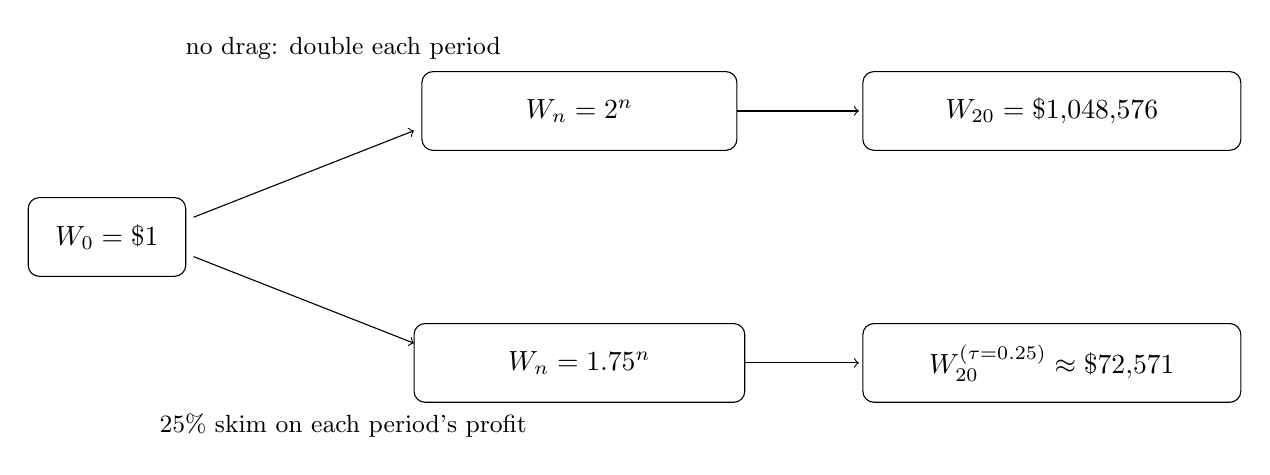
\begin{tikzpicture}[x=1cm,y=1cm]
\node[draw, rounded corners, minimum width=2cm, minimum height=1cm] (start) at (0,0) {\(W_0=\$1\)};
\node[draw, rounded corners, minimum width=4cm, minimum height=1cm] (top) at (6,1.6) {\(W_n=2^n\)};
\node[draw, rounded corners, minimum width=4.2cm, minimum height=1cm] (bottom) at (6,-1.6) {\(W_n=1.75^n\)};
\node[draw, rounded corners, minimum width=4.8cm, minimum height=1cm] (topend) at (12,1.6) {\(W_{20}=\$1{,}048{,}576\)};
\node[draw, rounded corners, minimum width=4.8cm, minimum height=1cm] (botend) at (12,-1.6) {\(W_{20}^{(\tau=0.25)}\approx \$72{,}571\)};

\draw[->] (1.1,0.25) -- (3.9,1.35);
\draw[->] (1.1,-0.25) -- (3.9,-1.35);
\draw[->] (8,1.6) -- (9.55,1.6);
\draw[->] (8.1,-1.6) -- (9.55,-1.6);

\node at (3,2.4) {\small no drag: double each period};
\node at (3,-2.4) {\small \(25\%\) skim on each period's profit};
\end{tikzpicture}
\caption{Transcript-based reconstruction of the lecture's compounding comparison. The drag does not merely subtract a little each round; it changes the growth factor itself.}
\end{figure}

\subsection{Question \& Answer}

\paragraph{Question.}
Why can a small recurring drag destroy almost the entire endpoint of compounding?

\paragraph{Answer.}
Because compounding does not act on a fixed quantity. It acts on a growing base. Once we slow the growth of the base in every round, every later round inherits that damage. The important theft is therefore not the first subtraction by itself, but the fact that all future doublings happen on a diminished platform. That is why a drag that looks modest locally becomes catastrophic globally.

The lecture is not finished once the arithmetic lands. It immediately turns the same logic into negotiation. The final speaker says that business negotiations are won by people who do not need the deal. He then complicates that line by admitting that real situations often involve genuine need. The example he gives is a negotiation stretching over roughly eight to nine months:
\begin{equation}
\Delta t_{\text{deal}}\approx 8\text{ to }9\ \text{months}.
\end{equation}
Late in the process, investors demand a clause he does not want. Lawyers and bankers are present. Large sums are at stake. He asks for a break, steps out, and tells his own side that the deal may be off. They think he is mad.

The key move comes when he returns and reframes the situation. He does not argue merely about the clause in isolation. He asks what kind of CEO they want after the deal closes. If he caves on something bad for shareholders now, what kind of representative of shareholder interests will he be tomorrow? The lecture's decision rule can be written schematically as
\begin{equation}
\text{if }U_{\text{shareholders}}(\text{accept clause})
<
U_{\text{shareholders}}(\text{walk away}),
\text{ reject the deal.}
\end{equation}
This is not literal lecture notation, but it preserves the logic exactly. The issue is not masculine bravado for its own sake. It is fiduciary alignment. He says, in effect, that the other side may have the money, but he has the willingness to refuse a bad deal. Then he falls quiet. The silence matters. It lets the reframing work.

By the end of the story, the lecture has braided arithmetic and conduct into one line of thought. Compounding is preserved by protecting the base. Shareholder value is preserved by refusing terms that corrode the enterprise after the deal is signed. The same instinct governs both: do not destroy the long run for a local concession.

\section{Summary}

The lecture begins with supercars and ends with compounding, but the path between them is consistent. First we are shown wealth as an object. Then the lecture peels away the object and gives us counted failure, partner risk, self-imposed discipline, sacrifice of the present self, dull but powerful land-backed businesses, negotiation sequencing, and finally a compact numerical proof that recurring drag can gut the endpoint of growth. If there is a single through-line, it is that wealth in this lecture is never treated as pure display. It is treated as a consequence of structure: what business we choose, what losses we survive, how we price our future, how we negotiate when pressured, and whether we understand the mathematics of what slowly compounds and what silently leaks away.